\chapter{Gläser}
\section{Anforderungen und Ziele}
Der Weinschorle-Automat soll eine Vielfalt verschiedener Glasformen erkennen um vor dem Befüllen dem Glas ein vordefiniertes Volumen zuordnen können. Ziel dieser Aufgabe ist das Vertraut machen mit Python an sich und insbesondere mit dem Skript, welches bereits in der Cloud für die Zuordnung zuständig ist.

\section{Ausgangssituation}
\begin{wrapfigure}{rt}{0.6\linewidth}
	\centering
	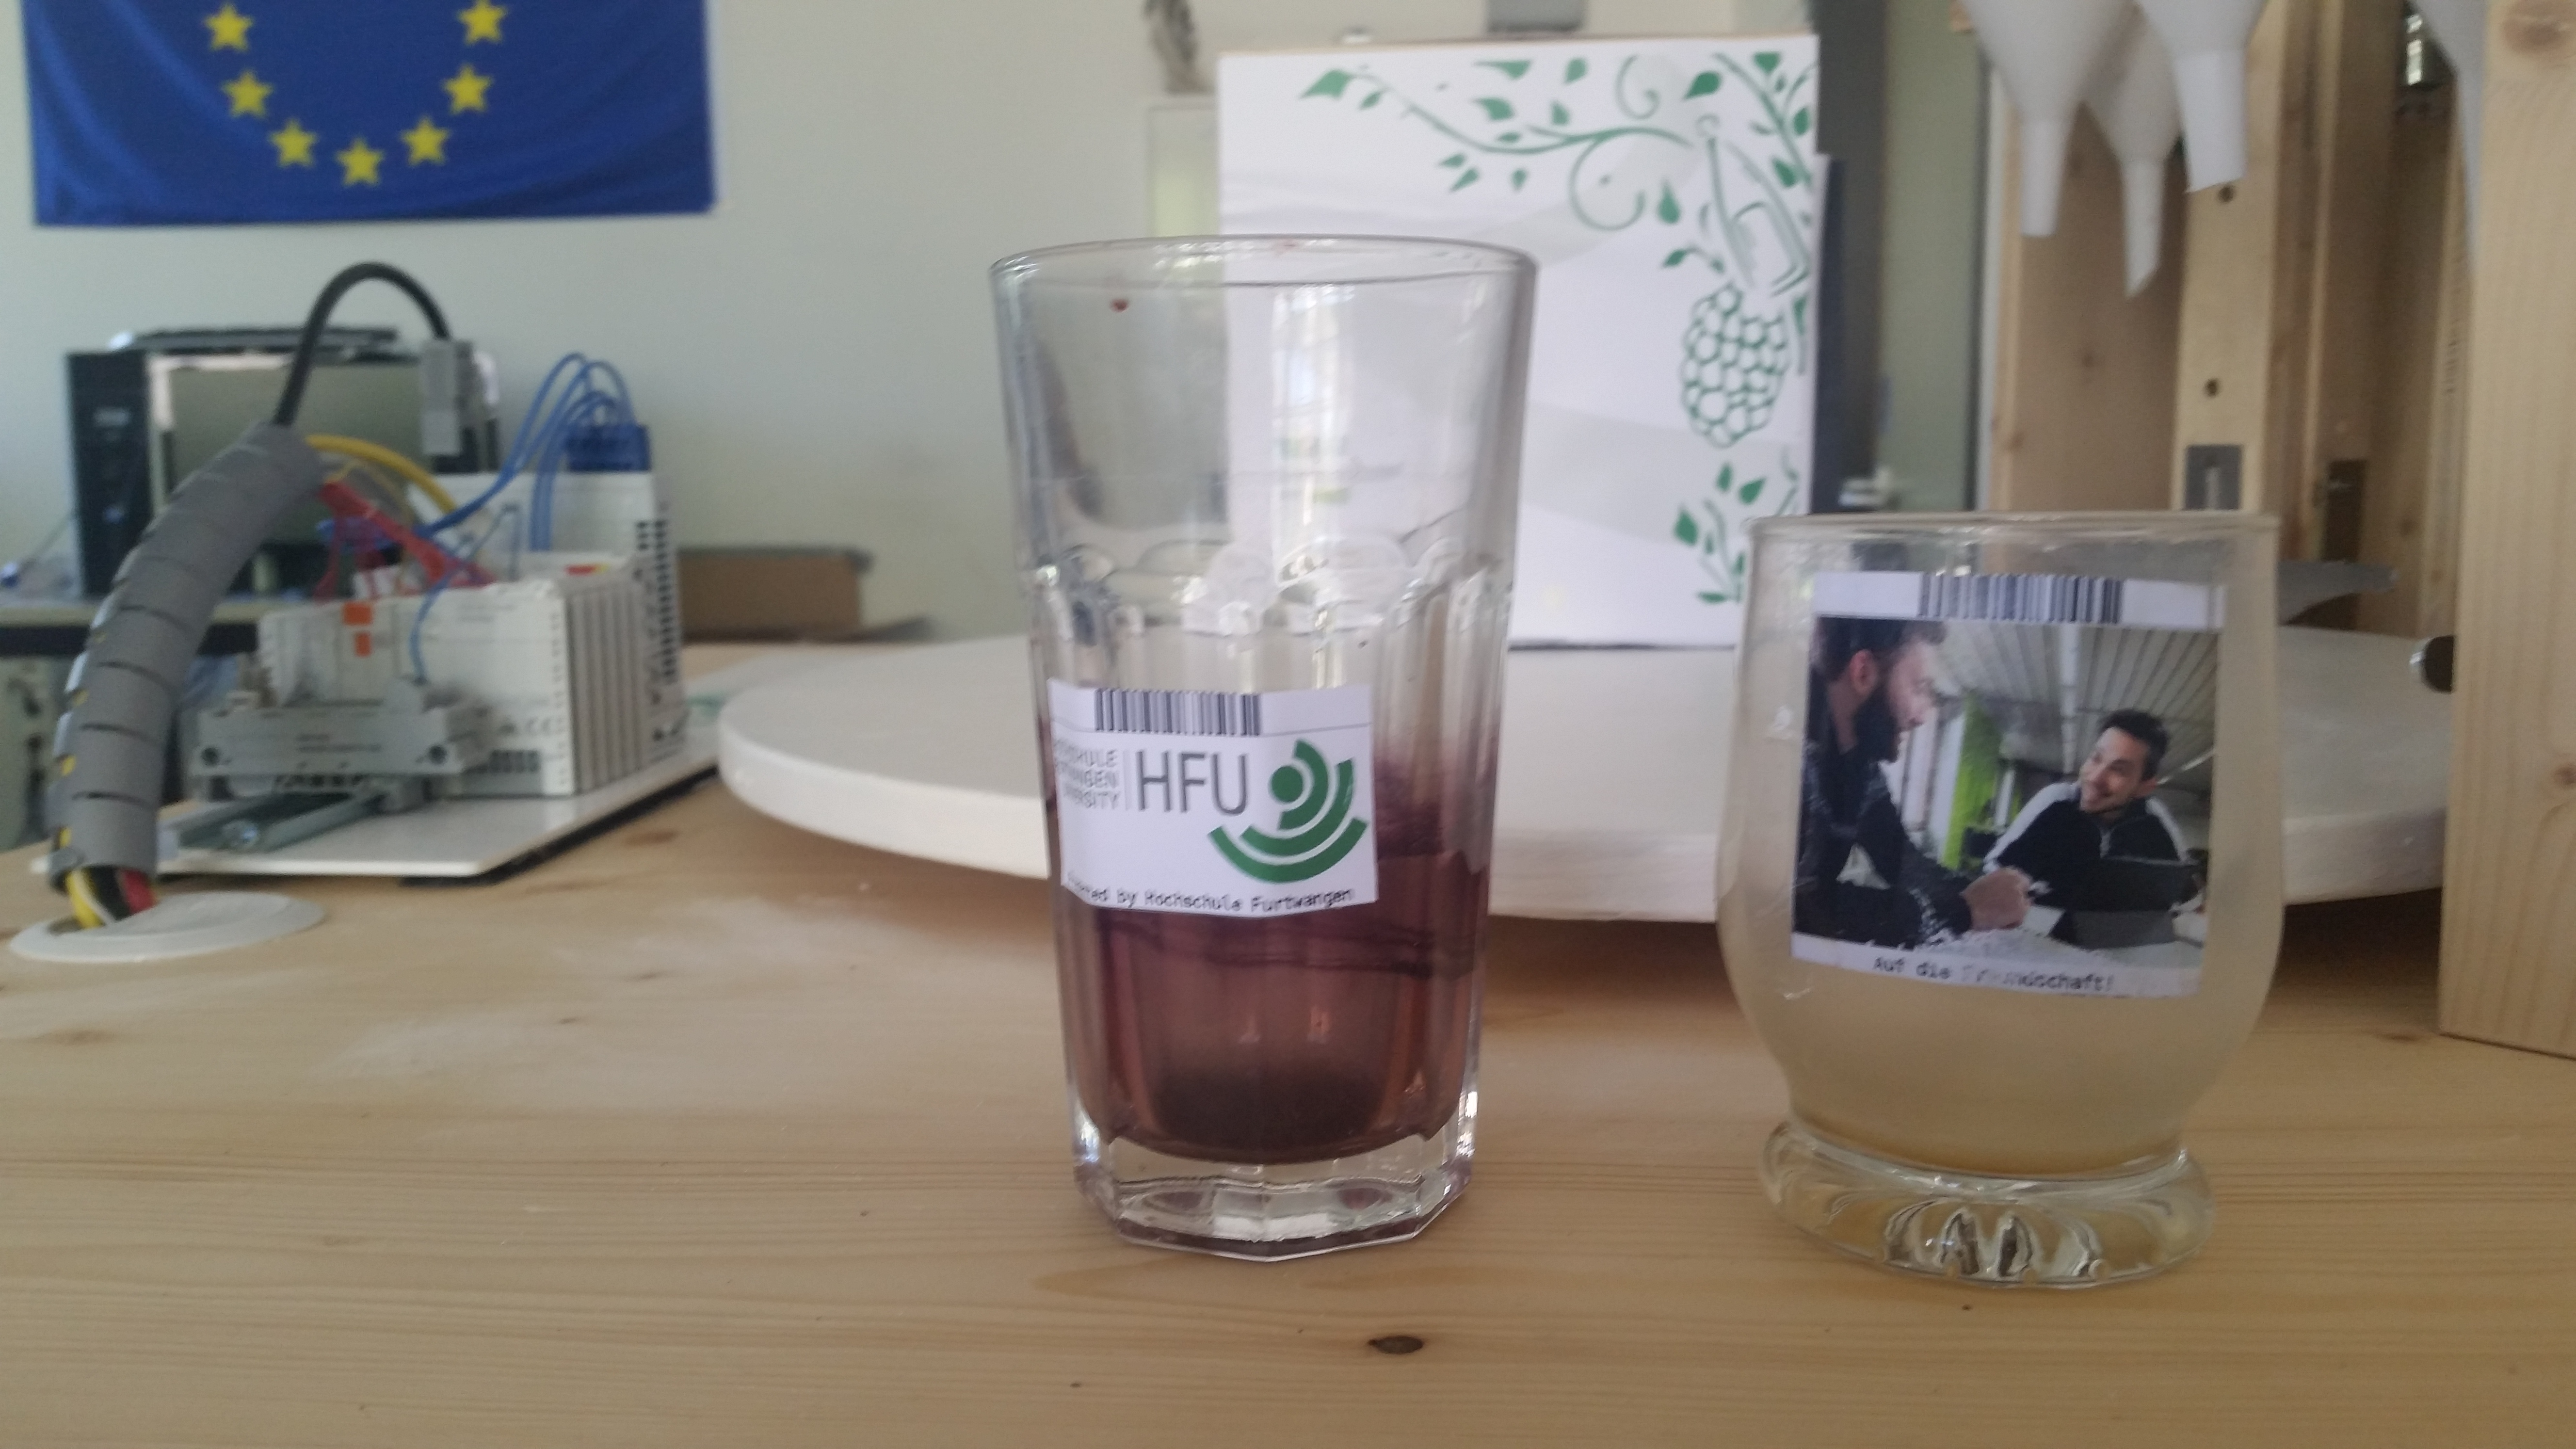
\includegraphics[width=\linewidth]{content/pictures/urspruengliche_glaeser}
	\caption{Ursprünglich bekannte Gläser}
	\label{fig:urspruengliche_glaeser}
	
	\centering
	\includegraphics[width=\linewidth]{content/pictures/position_der_kamera}
	\caption{Position der Kamera}
	\label{fig:kamera_position}
\end{wrapfigure}
Der Automat kann zu Beginn des Projekts bereits zwischen zwei unterschiedlichen Glastypen unterschieden (siehe Abbildung \ref{fig:urspruengliche_glaeser}). Dazu nimmt eine vertikal in der Fotokammer angebrachte Kamera (siehe Abbildung \ref{fig:kamera_position}) ein Bild des eingestellten Glases auf, welches zunächst zur Performance-Verbesserung auf ein kleineres Format zugeschnitten wird. Dieses Bild wird als Eingabe für das \ac{CNN} übergeben. Als Ausgabe wird das Glas im Automaten mit einer gewissen Wahrscheinlichkeit einem der beiden bekannten Glasformen zugeordnet. Basierend auf diesem Ergebnis wird die Befüll-Routine durchgeführt.
\clearpage

\section{Vorgehen}
\subsection{Trainingsdaten sammeln}
\begin{figure}[!h]
	\centering
	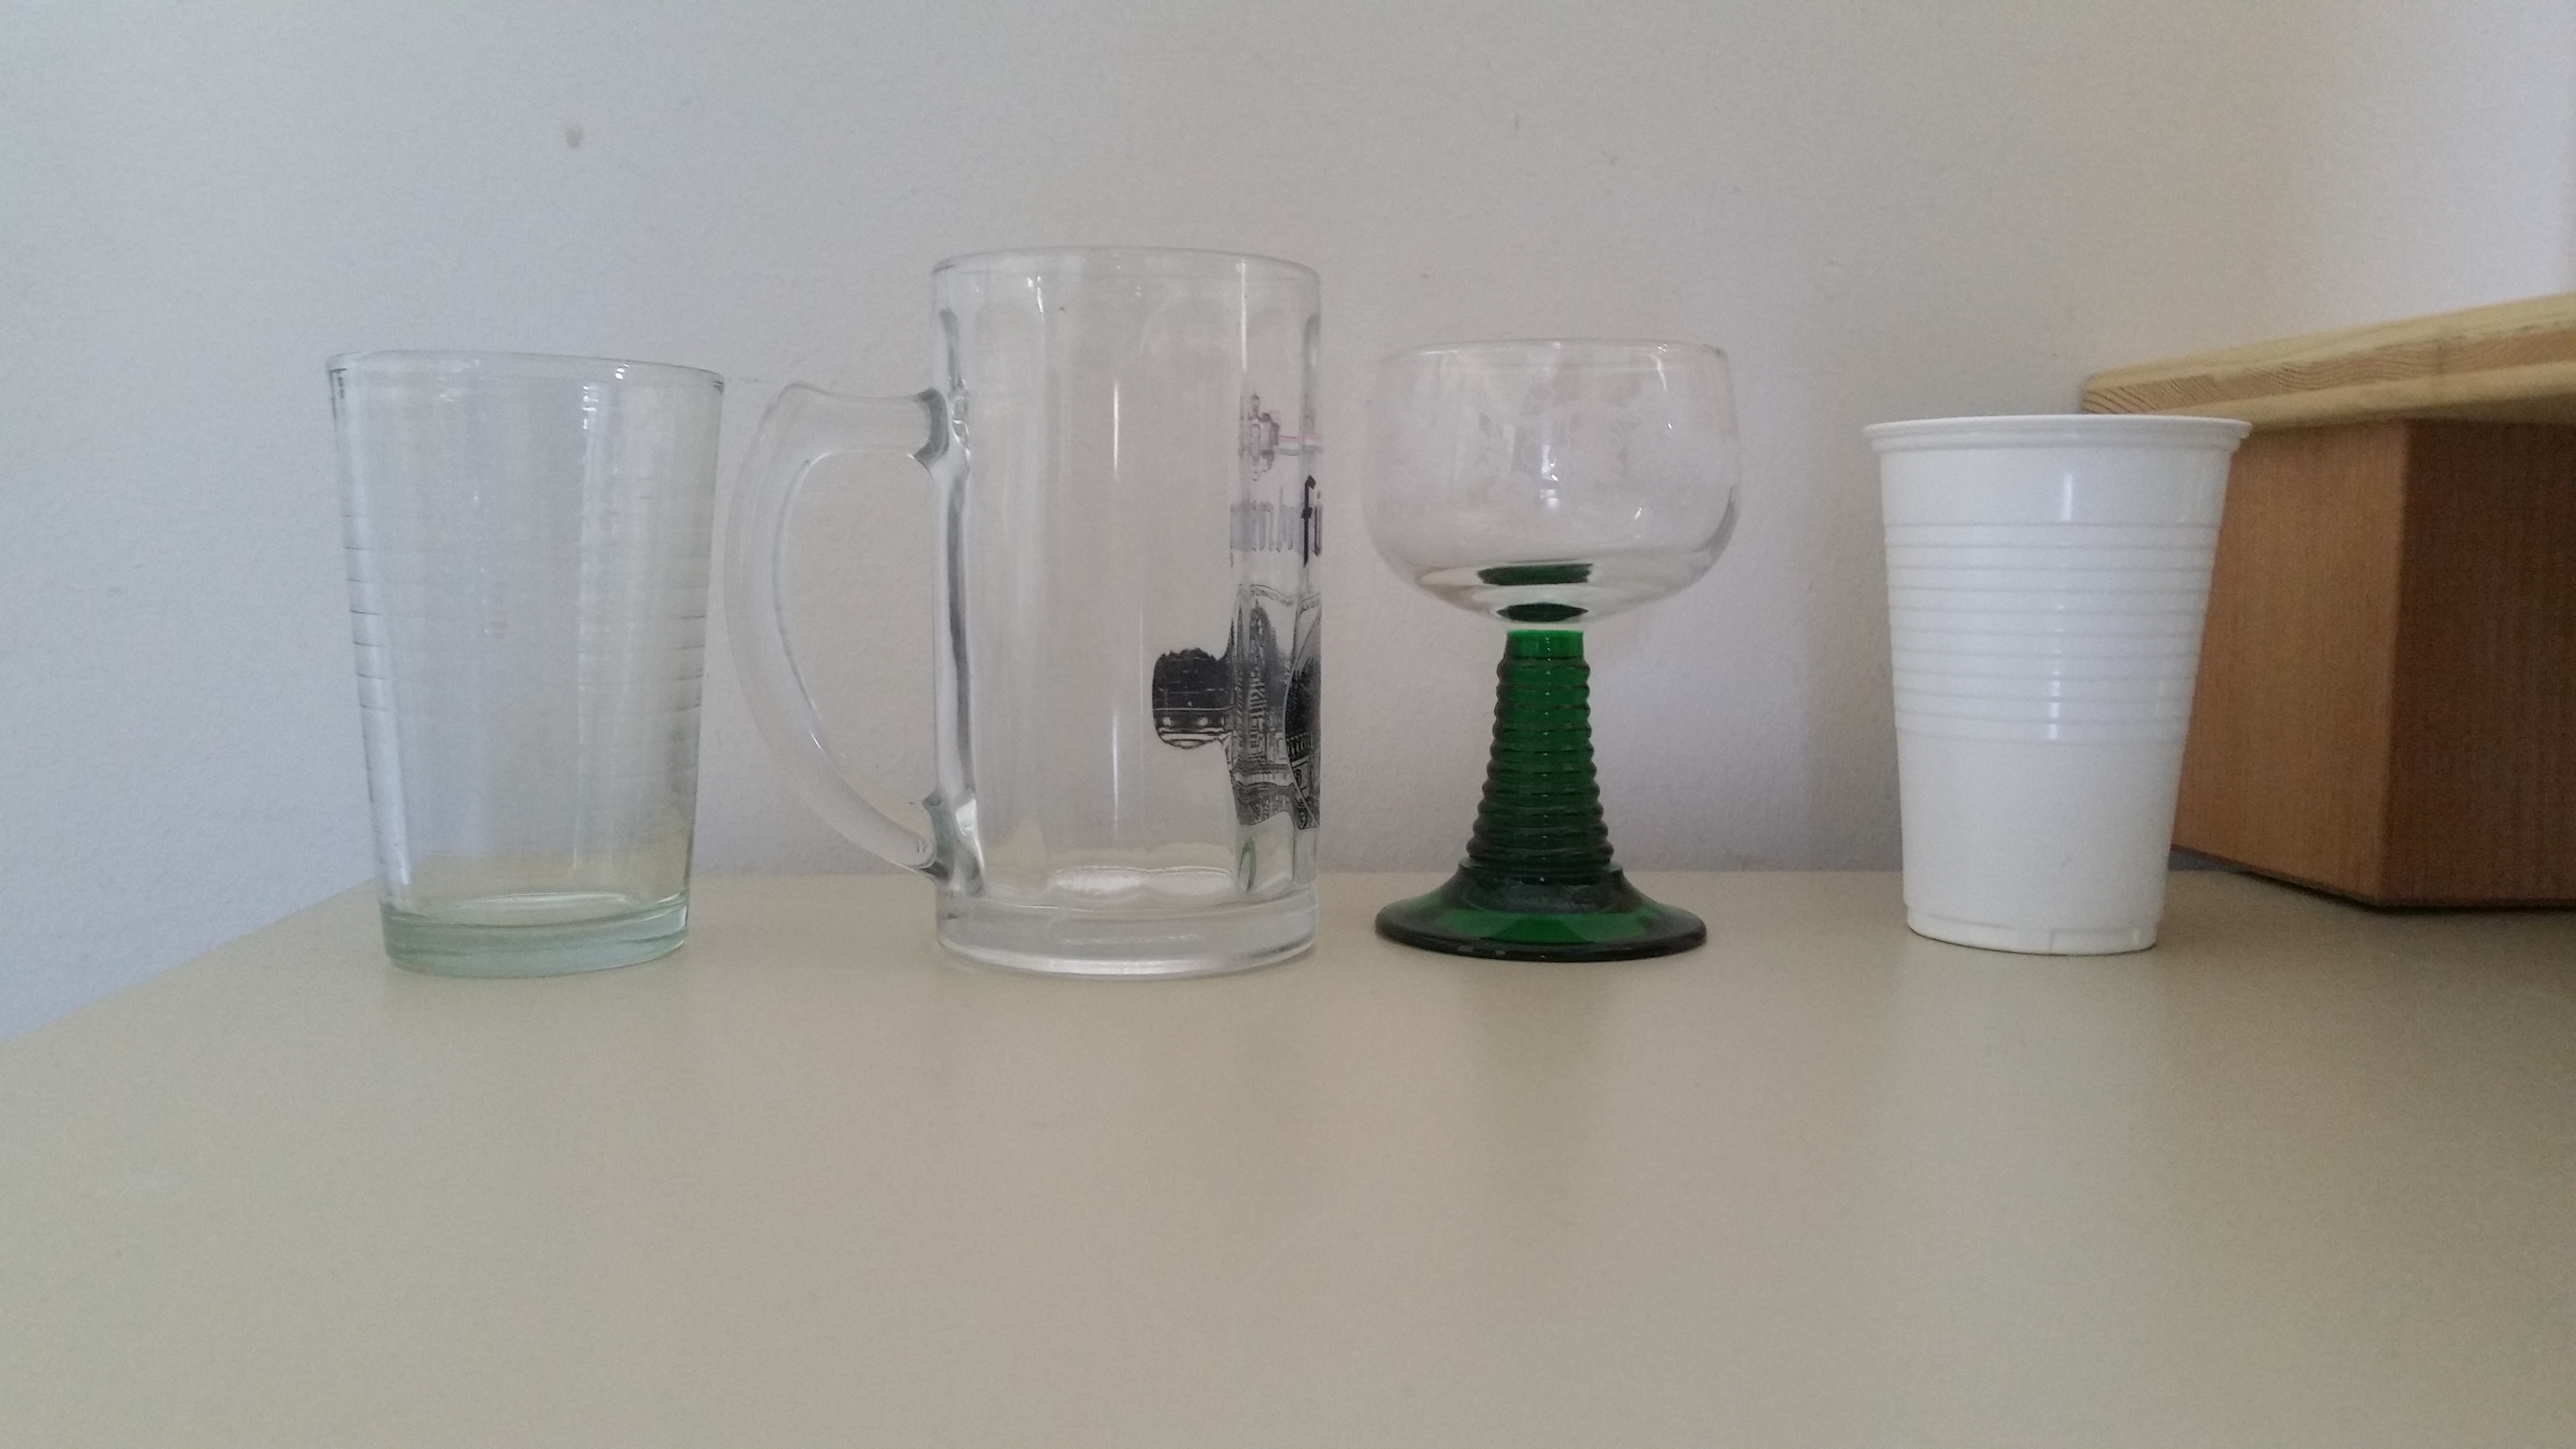
\includegraphics[width=0.7\linewidth]{content/pictures/neue_glaeser}
	\caption{Neue Gläser}
	\label{fig:neue_glaeser}
\end{figure}
Zunächst wurde die Kamera von dem Weinschorle-Automat getrennt und direkt an einen Laptop angeschlossen. Über diesen haben wir automatisch eine Serie von 100 Bildern für insgesamt vier neue Glasformen (siehe Abbildung \ref{fig:neue_glaeser}) aufgenommen. Zwischen den Aufnahmen war jeweils eine Verzögerung von drei Sekunden, so dass wir das Glas zwischen den Aufnahmen drehen konnten. Dadurch haben wir ein diverses Trainingsdatenset erzeugt, was die Trainingseffektivität des \ac{CNN} verbessert. 

\subsection{Trainingsdaten und Script anpassen}
Bevor wir das \ac{CNN} mit diesen Daten trainieren konnten mussten wir die Bilder zuschneiden (siehe Abbildung \ref{fig:vergleich_glas_zuschnitt}). Dies geschah mit dem selben Python-Script, welches bereits in der Routine des Weinschorle-Automaten verwendet wird. Weiterhin mussten wir das Trainingsscript dahingehend anpassen, dass wir die neuen Trainingsdaten als solche deklarieren und jedem Trainingsset ein entsprechendes Label zuordnen.

Damit hat sich die Anzahl der klassifizierbaren Gläser auf insgesamt sechs erhöht. Deshalb mussten wir im Predict-Script die Dimension des Output-Tensors an die neue Anzahl der Klassen entsprechend anpassen.

\begin{figure}
	\centering
	\fbox{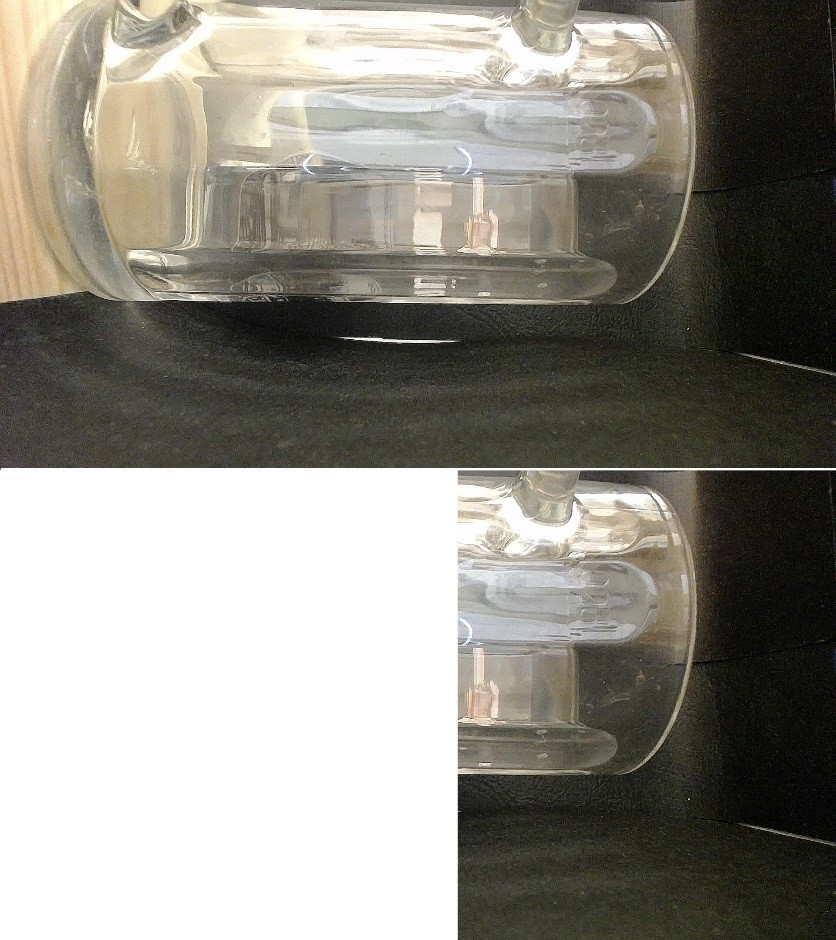
\includegraphics[width=0.7\linewidth,angle=90]{content/pictures/vergleich_glas_zuschnitt}}
	\caption{Foto vor (a) und nach (b) dem Zuschneiden}
	\label{fig:vergleich_glas_zuschnitt}
\end{figure}